\chapter{Results}

\section{calculation details} \label{sec::res::calc_det}

In this first investigation of the extraction of excited state form-factors using distillation, we restrict ourselves to a single ensemble of gauge-field configurations, having three degenerate flavors of dynamical quarks tuned to approximately the physical strange quark mass. This set of anisotropic Clover\footnote{Some details, including a brief derivation of the action may be found in \appref{app::Clover}.} lattices \cite{Edwards:2008ja, Lin:2008pr} has been used previously in studies of the meson spectrum \cite{Dudek:2009qf,Dudek:2010wm,Dudek:2011tt,Liu:2012ze,Dudek:2013yja}, meson decay constants~\cite{Mastropas:2014fsa}, baryon spectrum \cite{Edwards:2011jj, Dudek:2012ag, Edwards:2012fx, Padmanath:2013zfa} and meson-meson scattering \cite{Dudek:2010ew,Dudek:2012gj,Dudek:2012xn,Dudek:2014qha}. For the calculations reported on in this paper, we used 535 configurations of lattice volume $(L/a_s)^3 \times (T/a_t) = 16^3\times 128$, with a spatial grid spacing of $a_s \sim 0.12\, \mathrm{fm}$ and a temporal spacing roughly 3.5 times smaller. 

In this calculation we have an exact $SU(3)$ flavor symmetry such that all the octet mesons ($\pi$, $K$, $\eta$) are degenerate with a mass close to $700$ MeV. Where results are expressed in dimensionful units, they are determined from the dimensionless quantities $a_t E$ using the scale-setting procedure,
\begin{equation*}
E = \frac{a_t E}{a_t m_\Omega} \cdot m_\Omega^{\mathrm{phys.}}.
\end{equation*}
where $a_t m_\Omega$ is the $\Omega$ baryon mass calculated on this lattice and $m_\Omega^{\mathrm{phys.}}$ is the experimental value \cite{PDG-2012}.



\section{Extracted form-factors \& transitions\label{sec::results}}

In this section we present form-factors and transitions for the lightest few isovector pseudoscalar and vector mesons. We make use of the current ${  j^\nu = +\frac{2}{3}\bar{u}\gamma^\nu u -\frac{1}{3}\bar{d}\gamma^\nu d -\frac{1}{3}\bar{s}\gamma^\nu s  }$, such that the form-factors are in units of $e$, the magnitude of the electron charge. This calculation is performed with three flavors of dynamical quark all having the same mass, tuned approximately to the physical strange quark mass. We extract vector current matrix elements between ${(I,I_z) = (1,+1)}$ members of $SU(3)_F$ octets. Disconnected diagrams do not contribute to the amplitudes considered in this analysis as demonstrated in the appendix of \cite{Shultz:2015pfa}, where the flavor structure of the current is explored further.


%%%%%%%%%%%%%%%%%%%%%%%%%%%%%%%%%%%%%%%%%%%%%%%%%
%%% FORM-FACTORS
%%%%%%%%%%%%%%%%%%%%%%%%%%%%%%%%%%%%%%%%%%%%%%%%%

\subsection{Form-factors}


\subsubsection{$\pi$ form-factor}

The pion form-factor appears in the matrix element decomposition, $\big\langle \pi^+(\vec{p}\,') \big| j^\mu \big| \pi^+(\vec{p}) \big\rangle = (p+p')^\mu \, F_\pi(Q^2)$, which we will extract from three-point Euclidean correlation functions computed using optimized ground-state pion operators of definite momentum at the source (at $t=0$) and the sink (at $\Delta t = 28\, a_t$). As discussed previously, we will present $F(Q^2;t)$, where the leading Euclidean time-dependence of the correlation function has been removed, with any remaining time-dependence signaling the presence of excited state contributions to the correlation function. By utilizing many values of $\vec{p}$ and  $\vec{p}\,'$ we can determine the form-factor at a range of $Q^2$ values. We plot $F_\pi(Q^2;t)$ for a subset of these $Q^2$ values in Figure~\ref{fig::pion_proj0_pion_proj0_Q2_dep}, where for each $Q^2$ we overlay a fit according to the form in \eqnref{three_point_fit}.

\afterpage{
\begin{figure}[htbp]
\begin{centering}
  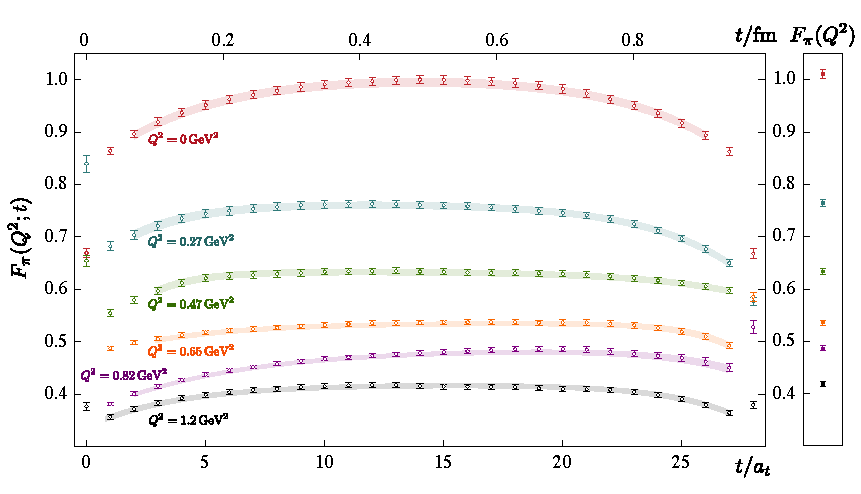
\includegraphics[width=0.8\linewidth]{figures/radTrans/pion_proj0_pion_proj0_Q2_dep.pdf}
  \caption{ Typical $F_\pi(Q^2; t)$ extracted from optimized three-point functions (points) with fit descriptions using \eqnref{three_point_fit} (curves). Note that the data points have a high degree of timeslice correlation which is accounted for in the fitting.  \label{fig::pion_proj0_pion_proj0_Q2_dep}}
    \end{centering}
\end{figure}
\clearpage
}

\afterpage{
\begin{figure}[htbp]
\begin{centering}
  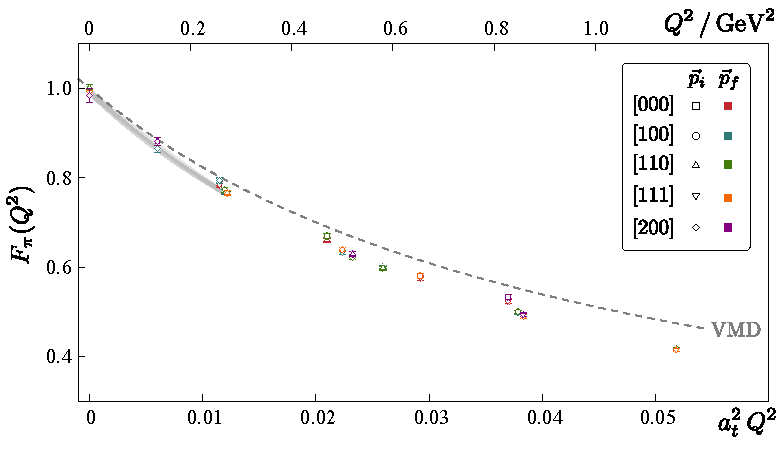
\includegraphics[width=0.8\linewidth]{figures/radTrans/pion_proj0_pion_proj0.pdf}
  \caption{ Pion ground-state form-factor, $F_\pi(Q^2)$, using the improved current, see \secref{app::Clover}. Vector meson dominance using the $\rho$ meson mass on this lattice shown by the dashed curve. Fits to the small-$Q^2$ points using gaussian and single-pole forms shown by the gray curves. \label{fig::pion_formfactor} }
    \end{centering}
\end{figure}
\clearpage
}


In Figure~\ref{fig::pion_formfactor} we plot the resulting $Q^2$ dependence, shown via both dimensionless $a_t^2 Q^2$ and scale-set using the $\Omega$-baryon mass prescription presented in \secref{sec::res::calc_det}. A large number of kinematic points are sampled by considering all combinations of momentum such that $n^2_{\vec{p}} \le 4$, $ n^2_{\vec{p}\,'} \le 4$ and $ n^2_{\vec{q}} \le 4$. The extracted points appear to lie on a single curve, with only small residual scatter which can originate from fitting-range systematics and modest discretization effects.

Describing the $Q^2$ dependence may offer some phenomenological insight, albeit in this calculation at an unphysically heavy quark mass. A commonly used approach to describe vector-current form-factors of hadrons is to argue that the photon is behaving like the lightest vector meson which can couple to the hadrons in question, which in this case would be the $\rho$. This ``vector meson dominance"(VMD) describes the $Q^2$ dependence by ${F_{\mathrm{VMD}}(Q^2) = \frac{1}{1 + Q^2/m_\rho^2 }}$. Using the $\rho$ mass determined on these lattices, $m_\rho = 1020(1)\, \mathrm{MeV}$, we have the dashed curve shown in Figure~\ref{fig::pion_formfactor}, which is seen to describe the lattice data reasonably well only for small photon virtualities. One possible explanation of this effect is that as we move out to larger $Q^2$, considering only the nearest time-like pole, the $\rho$, and neglecting all excitations, becomes a progressively poorer approximation.

 
The distribution of charge within the pion can be characterized by the \emph{charge radius}, defined via the slope of the form-factor at zero virtuality, ${\langle r^2 \rangle \equiv -6 \frac{d}{dQ^2}F(Q^2) \big|_{Q^2=0}}$. We may obtain this quantity from the discrete $Q^2$ data presented in Figure~\ref{fig::pion_formfactor} by parameterizing the $Q^2$--dependence for small virtualities. Considering gaussian ${ \big(  F_\pi(Q^2) = F(0)\, e^{-Q^2/16\beta^2}  \big) }$ and pole ${ \big(  F_\pi(Q^2) = F(0)\, \tfrac{1}{1 + Q^2/m^2} \big) }$ forms to describe ${Q^2 < 0.3\,\mathrm{GeV}^2}$, we obtain\footnote{If $F(0)$ is allowed to float in fits, a value statistically compatible with 1 is obtained, as it must since the pion form-factor at zero $Q^2$ was used to set $Z_V$. The fit $\chi^2$ values obtained are fairly large due to the scatter in the statistically precise data, which is likely due to small discretization effects which are not described by these smooth fit-forms.} 
a charge radius ${  \langle r^2 \rangle_{\pi}^{1/2} = 0.47(6) \; \mathrm{fm}  }$, where the error includes the variation over fit-form. As we might expect, in a calculation where three flavors of quarks all have approximately the strange quark mass, we obtain a pion charge radius somewhat smaller than the physical pion ${\langle r^2 \rangle_\pi^{1/2} = 0.67(1)\,\mathrm{fm}}$ \cite{Amendolia:1986wj, PDG-2012}, and also smaller than the physical kaon ${  \langle r^2 \rangle_K^{1/2} = 0.58(4) \, \mathrm{fm}  }$ \cite{Amendolia:1986ui}.








%%%%%%%%%%%%%%%%%%%%%%%%%%%%%%%%%%%%%%%%%%%%%%%%%%%%%%%%%%%%%%%%%%%%%%%%%%%%%%%%%%%%%%%%%%%
%%%%%%%%%%%%%%%%%%%%%%%%%%%%%%%%%%%%%%%%%%%%%%%%%%%%%%%%%%%%%%%%%%%%%%%%%%%%%%%%%%%%%%%%%%%
\subsubsection{$\rho$ form-factors}



The three form-factors required to describe the vector-current response of a vector hadron may be defined as in \eqnref{eqn::rho_Gmultipole_basis}, which makes use of a multipole basis. The decomposition presented in \eqnref{eqn::rho_Gi_basis} defines the linear system which we may solve, as described in \secref{sec::FFExtract}, for the form-factors. We plot the charge, $G_E(Q^2)$, magnetic, $G_M(Q^2)$, and quadrupole, $G_Q(Q^2)$ form-factors in Figure~\ref{fig::rho_form_factors}. Examination of Equations~\ref{eqn::rho_Gi_basis}, \ref{eqn::rho_Gmultipole_basis} indicates that only the charge form-factor has a non-zero kinematic factor when $Q^2=0$, and as such only it is determined there, while all three form-factors are sampled for positive non-zero $Q^2$. The smallest form-factor, $G_Q$, shows the largest scatter, which likely originates from modest discretization effects and timeslice fitting-range fluctuations.

\afterpage{
\begin{figure}[htbp]
\begin{centering}
  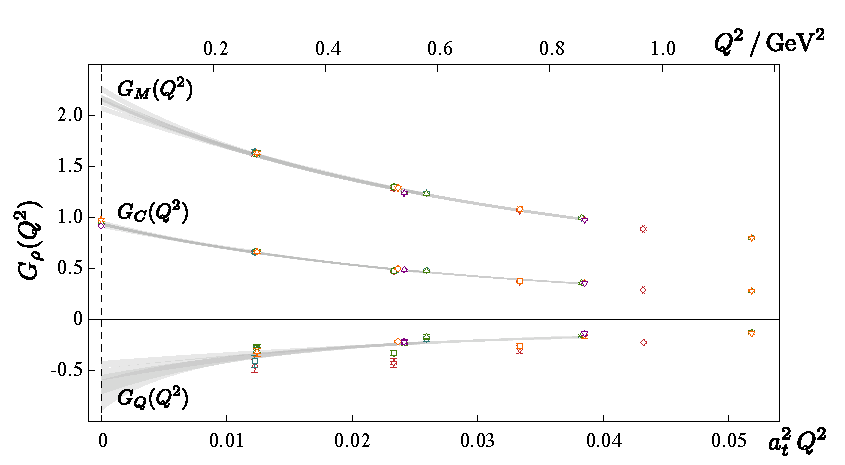
\includegraphics[width=0.80\linewidth]{figures/radTrans/rho0_rho0.pdf}
  \caption{ Ground-state $\rho$ meson multipole form-factors. Points have the same color and shape labeling presented in Figure~\ref{fig::pion_formfactor}. Fits to the $Q^2$ dependence, described in the text, are shown as gray curves. \label{fig::rho_form_factors}}
    \end{centering}
\end{figure}
\clearpage
}


Fitting the $Q^2$ dependence of the charge form-factor with various forms\footnote{$G(0) e^{-Q^2/16\beta^2}$, $G(0) e^{-Q^2(1+\alpha Q^2)/16\beta^2}$, $G(0)/(1+ Q^2/m^2)$, $G(0)/(1+ Q^2/m^2 + \gamma (Q^2/m^2)^2 )$, $G(0) \frac{e^{-Q^2/16\beta^2}  }{1+Q^2/m^2}$ }, over various $Q^2$ ranges we obtain $G_C(0) = 0.94(1)$ and ${  \langle r^2 \rangle_\rho^{1/2} = 0.55(5) \, \mathrm{fm} }$ where the errors include a systematic variation over different fit forms. The deviation of the charge from 1 was discussed previously \secref{sec::Renormalization}. 

In order to determine the magnetic and quadrupole moments from $G_M(0)$ and $G_Q(0)$ it is necessary to parameterize the $Q^2$ dependence of the form-factors and extrapolate back to $Q^2=0$. Utilizing a range of possible forms, we obtain ${G_M(0) = 2.17(10)}$ and ${G_Q(0) = -0.54(10)}$, accounting for the variation over fit-forms, which is much larger than the statistical uncertainty, in the errors. More precise determinations of these quantities could be obtained if twisted boundary conditions were used to sample the form-factors at smaller $Q^2$ (see for example \cite{Flynn:2005in}).

Within a simple picture of the $\rho$ as a $q\bar{q}$ bound-state, the presence of a quadrupole moment would indicate a required admixture of $D$-wave into the dominantly $S$-wave wavefunction. Previous estimates of the $\rho$-meson magnetic moment in versions of QCD with heavier than physical quarks come from chiral effective theory \cite{Djukanovic:2013mka} where $G_M(0) \sim 2.2$ for large pion masses, and quenched lattice QCD using either an energy shift in a magnetic field \cite{Lee:2008qf} where $G_M(0) = 2.13(6)$, or extrapolation to zero $Q^2$ from a single spacelike virtuality \cite{Hedditch:2007ex} where $G_M(0) = 2.05(4)$, at comparable unphysical pion masses. A dynamical calculation, Ref.~\cite{Owen:2015gva}, which appeared while this manuscript was in the final stages of production, found, at a comparable pion mass, $G_M(0) = 2.23(2)$ and $G_Q(0) = -0.362(20)$, using a model extrapolation to $Q^2=0$ from a single non-zero $Q^2$ point.




%%%%%%%%%%%%%%%%%%%%%%%%%%%%%%%%%%%%%%%%%%%%%%%%%%%%%%%%%%%%%%%%%%%%%%%%%%%%
%%%%%%%%%%%%%%%%%%%%%%%%%%%%%%%%%%%%%%%%%%%%%%%%%%%%%%%%%%%%%%%%%%%%%%%%%%%%
%%%%%%%%%%%%%%%%%%%%%%%%%%%%%%%%%%%%%%%%%%%%%%%%%%%%%%%%%%%%%%%%%%%%%%%%%%%%

\subsubsection{$\pi'$ form-factor}

\afterpage{
\begin{figure}[htbp]
\begin{centering}
  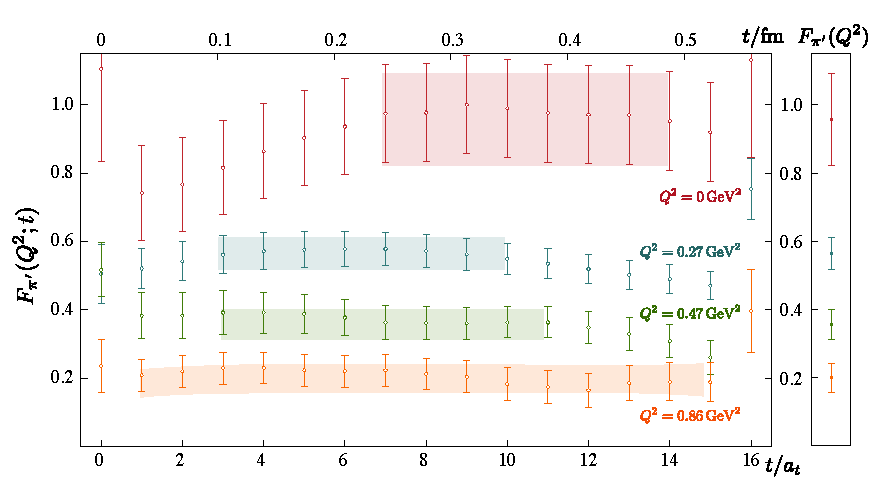
\includegraphics[width=0.8\linewidth]{figures/radTrans/pion_proj1_pion_proj1_Q2_dep.pdf}
  \caption{Current insertion time dependence for the form-factor of the first excitation of the pion, $F_{\pi'}(Q^2;t)$, shown for a range of source and sink momenta. The high degree of timeslice-timeslice data correlation  is manifested in the error on the fit which is not significantly reduced relative to the error on the individual data points. \label{fig::pion_proj1_pion_proj1_Q2_dep}}
    \end{centering}
\end{figure}
\clearpage
}

\afterpage{
\begin{figure}[htbp]
\begin{centering}
  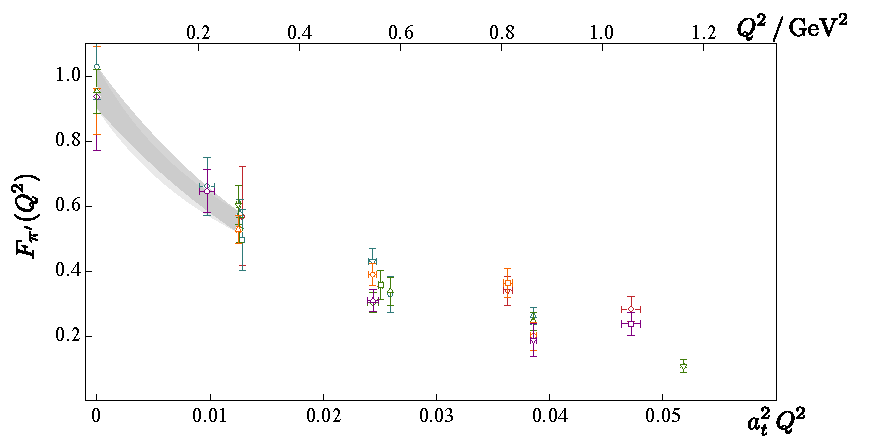
\includegraphics[width=0.8\linewidth]{figures/radTrans/pion_proj1_pion_proj1.pdf}
  \caption{First-excited pion form-factor, $F_{\pi'}(Q^2)$. Points have the same color and shape labeling presented in Figure~\ref{fig::pion_formfactor}. Fits to low $Q^2$ dependence used to constrain charge-radius, as described in text, shown as gray bands.  
  \label{fig::piStar_form_factor}}
    \end{centering}
\end{figure}
\clearpage
}



The examples presented in the previous two subsections were the lightest states with the relevant quantum numbers. As such it was not strictly necessary to use optimized operators -- any suitable meson interpolators used in the three-point functions will, in the limit of large time separations, give access to the matrix elements. We will now move to the case of an excited state, the first excitation of the pion, which we access using optimized operators to eliminate the contribution of the ground-state pion.

As described in \chapref{chap::Spectroscopy}, the signals for excited states are typically noisier than those for the ground state, and as such we separate the source and sink operators by a smaller time, in this case $\Delta t = 16 \, a_t$. The decomposition for this matrix element is of the same form as the pion described previously, \eqnref{eqn::pion_decomp}. We plot the extracted form-factor, $F_{\pi'}(Q^2; t)$, as a function of the current insertion timeslice in Figure~\ref{fig::pion_proj1_pion_proj1_Q2_dep}. 



The $Q^2$ dependence of the form-factor, $F_{\pi'}(Q^2)$, is presented in Figure~\ref{fig::piStar_form_factor}. While the extracted values at $Q^2=0$ are not statistically precise, they are certainly consistent with unity. The charge radius can be extracted from the slope at $Q^2=0$ which we determine by parameterizing\footnote{Gaussian ($F_{\pi'}(0) \, e^{-Q^2/16\beta^2}$) and one-pole ($F_{\pi'}(0) / (1 + Q^2 / m^2 )$) forms were used. }
 the data for $Q^2 \lesssim 0.3\,\mathrm{GeV}^2$, yielding ${   \langle r^2 \rangle_{\pi'}^{1/2} = 0.74(6) \, \mathrm{fm} }$ where the error includes variation over parameterization form. As we might expect for a state which likely can be characterized as a radial excitation, this is significantly larger than the $0.47(6)\,\mathrm{fm}$ found for the ground-state pion at this quark mass. 
 
Ref.~\cite{Owen:2015gva}, computing at a very similar pion mass found $0.517(4)\,{\rm fm}$ for the ground-state pion charge radius, and $0.59(3)\,{\rm fm}$ for the first excitation of the pion. Their approach determines a single point on the form-factor curve at $Q^2\sim 0.16 \,\mathrm{GeV^2}$ which is used to determine the slope at $Q^2=0$ assuming monopole dependence on $Q^2$. 




%%%%%%%%%%%%%%%%%%%%%%%%%%%%%%%%%%%%%%%%%%%%%%%%%%%%%%%%%%%%%%%%%%%%%%%%%%%%%%%%%%%%%%%%%%%%%%%%%%%%%
%%%%%%%%%%%%%%%%%%%%%%%%%%%%%%%%%%%%%%%%%%%%%%%%%%%%%%%%%%%%%%%%%%%%%%%%%%%%%%%%%%%%%%%%%%%%%%%%%%%%%
%%%%%%%%%%%%%%%%%%%%%%%%%%%%%%%%%%%%%%%%%%%%%%%%%%%%%%%%%%%%%%%%%%%%%%%%%%%%%%%%%%%%%%%%%%%%%%%%%%%%%

\subsection{Radiative Transitions}



%%%%%%%%%%%%%%%%%%%%%%%%%%%%%%%%%%%%%%%%%%%%%%%%%%%%%%%%%%%%%%%%%%%%%%%%%%%%%%%%%%%%%%%%%%%%%%%%%%%%%
\subsubsection{$\pi' \rightarrow \pi \gamma$ transition}


In a transition between different pseudoscalar mesons, the decomposition of the current in terms of a form-factor $F_{\pi' \pi}(Q^2)$ is as in \eqnref{eqn::pipip_decomp}, and the form-factor must vanish at $Q^2=0$. The transition form-factor is extracted from three-point functions with $\Delta t = 20 \, a_t$, fitting the time-dependence as previously to account for any residual unwanted excited state contribution. We plot the extracted form-factor in \figref{fig::pi_pistar_transition} -- that we are now able to explore the timelike $Q^2$ region, where previously all points were spacelike, follows from the differing masses of the hadrons at source and sink, a simple example being the case where $\vec{p}\,' = \vec{p}$, so that ${Q^2 = - \big( E'(\vec{p}\,) - E(\vec{p}\,) \big)^2 < 0}$. In order to be able to trivially relate our Euclidean amplitudes to Minkowski amplitudes, we must restrict ourselves to the region where the current is not timelike enough to produce on-shell hadrons. In this calculation where the $\pi \pi$ threshold is above the $\rho$ mass, this limits us to ${  Q^2 > - m_\rho^2 \sim - 1\,\mathrm{GeV}^2  }$. In order to explore further into the timelike region, a somewhat more sophisticated approach must be followed \cite{Meyer:2011um, Feng:2014gba}.

\afterpage{
\begin{figure}[htbp]
\begin{centering}
  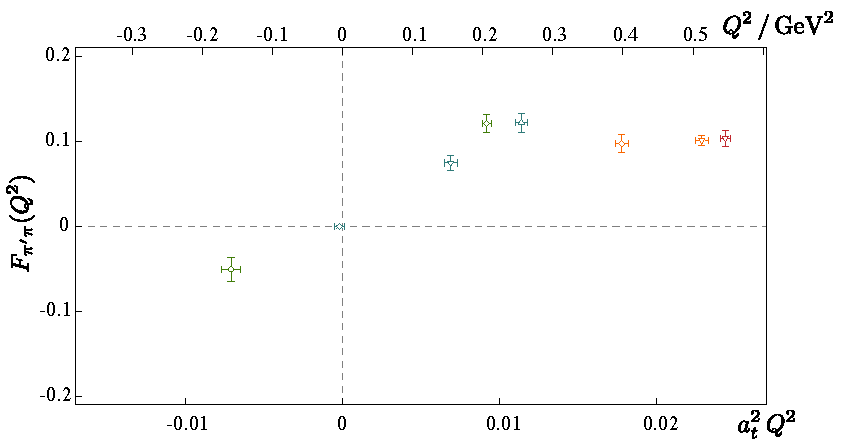
\includegraphics[width=0.8\linewidth]{figures/radTrans/pi_pistar_transition_formfactor.pdf}
  \caption{Transition form-factor between first-excited and ground-state pions, $\pi' \to \pi \gamma$. Points have the same color and shape labeling presented in Figure~\ref{fig::pion_formfactor} with the excited pion having momentum $\vec{p}_f$. \label{fig::pi_pistar_transition}}  \end{centering}
\end{figure}
\clearpage
}



%%%%%%%%%%%%%%%%%%%%%%%%%%%%%%%%%%%%%%%%%%%%%%%%%%%%%%%%%%%%%%%%%%%%%%%%%%%%%%%%%%%%%%%%%%%%%%%%%%%%%
\subsubsection{$\rho \rightarrow \pi \gamma$ transition}\label{rhopigamma}

A suitable decomposition for a vector to pseudoscalar transition in terms of a dimensionless form-factor is given in \eqnref{rho_pi_ff}. Using optimized operators for the ground-state $\rho$ and ground-state $\pi$ we computed correlation functions with $\Delta t = 28\, a_t$ for a large range of source and sink momenta -- the resulting determination of the form-factor, $F_{\rho \pi}(Q^2)$ is presented in Figure~\ref{fig::rho_pi_transition}.

The value of the form-factor at $Q^2=0$, known as the photocoupling, is of particular interest since it controls the rate of the physically allowed radiative transition process, $\rho^\pm \to \pi^\pm \gamma$. As can be seen in Figure~\ref{fig::rho_pi_transition}, we do not determine this quantity directly, but we may estimate it using interpolation between our space-like and time-like points. Using a range of fit forms over several $Q^2$ ranges (plotted in grey) we estimate $F_{\rho \pi}(0) = 0.494(8)$, where the error includes variation over fit-forms.


The Lorentz invariant matrix element for the decay $\rho^+ \to \pi^+ \gamma$ can be obtained by contracting the matrix element in \eqnref{rho_pi_ff} with a final state polarization vector, $\mathcal{M}_{\lambda_\gamma,\lambda} = \epsilon^*_\mu(\lambda_\gamma,\vec{q}) \big\langle \pi^+(\vec{p}\,') \big| j^\mu \big| \rho^+(\lambda, \vec{p}) \big\rangle$,
and for a vector stable under the strong interaction, we may obtain the decay width from
\begin{equation*}
\Gamma(\rho^+\rightarrow \pi^+\gamma) = \frac{1}{32\pi^2}\int \!\! d\Omega_{\vec{q}} \, \frac{\lvert \vec{q}\rvert}{m_\rho^2} \,  \frac{1}{3} \sum_{\lambda_\gamma,\lambda} \lvert \mathcal{M}_{\lambda_\gamma,\lambda}  \rvert^2,
\end{equation*}
where we have summed over the final state photon polarizations and averaged over the initial state polarization of the $\rho$. Using the decomposition above, and restoring the factors of $e$, we obtain the result relating the width to the photocoupling,
\begin{equation*}
\Gamma(\rho^+\rightarrow \pi^+\gamma) = \alpha\frac{4}{3} \frac{\lvert \vec{q} \rvert^3}{(m_\rho \!+\! m_\pi)^2} \lvert F_{\rho \pi}(0) \rvert^2,
\end{equation*}
where $\alpha = e^2/4\pi$. 

The calculation performed here uses three degenerate quark flavors tuned to approximate the physical strange quark mass and as such our photocoupling determination cannot be directly compared with experiment. For orientation we show in Figure~\ref{fig::rho_pi_transition}, the experimental values, $F_{\rho \pi}(0) = 0.33(2)$ and $F_{K^{\!*}\!K}(0) = 0.57(3)$ extracted from the corresponding decay rates obtained via the Primakoff effect for pions and kaons incident on nuclear targets \cite{PhysRevD.33.3199,Capraro:1987rp,PhysRevLett.51.168}.

\afterpage{
\begin{figure}[htbp]
\begin{centering}
  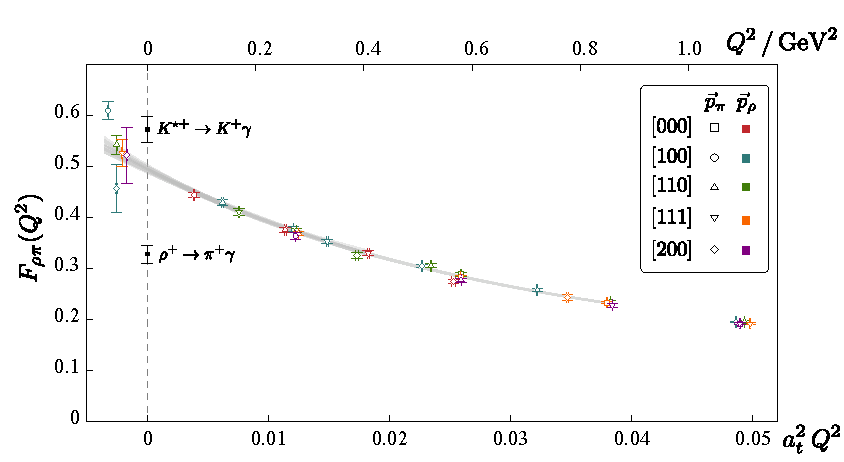
\includegraphics[width=0.8\linewidth]{figures/radTrans/pion_proj0_rho_proj0.pdf}
  \caption{Ground-state $\rho$ to ground-state $\pi$ transition form-factor. Curves in gray show fits used to interpolate between spacelike and timelike regions to determine the photocoupling, $F_{\rho\pi}(0)$. Experimental decay widths converted to photocouplings shown for orientation.  \label{fig::rho_pi_transition}}
    \end{centering}
\end{figure}
\clearpage
}

The $Q^2$ dependence of this meson transition form-factor plays a role in models of deuteron electromagnetic structure, where a virtual photon probe may couple to the bound nucleons or to the meson currents proposed to supply the binding \cite{Arnold:1979cg}.




%%%%%%%%%%%%%%%%%%%%%%%%%%%%%%%%%%%%%%%%%%%%%%%%%%%%%%%%%%%%%%%%%%%%%%%%%%%%%%%%%%%%%%%%%%%%%%%%%%%
\subsubsection{$\rho'\rightarrow\pi\gamma$ transition}
The first-excited $\rho$ state may also undergo a transition to the ground-state pion, with the form of the decomposition of the matrix element being the same as in the previous section. In \secref{sec::Spec:results} we presented the spectrum of excited vector mesons, finding that the first-excited state, $m_{\rho'} = 1882(11) \,\mathrm{MeV}$, is close to being degenerate with the second-excited state $m_{\rho''} = 1992(6) \,\mathrm{MeV}$. Our use of optimized operators corresponding to orthogonal combinations of basis operators allows us to reliably study the two excitations independently. 

We extract the form-factor using optimized operators in correlation functions with time-separation, $\Delta t = 20 \,a_t$, with the results presented in Figure~\ref{fig::rho1_pi_transition}. To determine the photocoupling, $F_{\rho' \pi}(0) = 0.050(4)$, we perform fits to the data over various $Q^2$ ranges using several fit-forms, and the quoted uncertainty includes this variation.

The photocoupling for this transition is observed to be an order of magnitude smaller than that of $\rho \to \pi \gamma$ extracted in Section~\ref{rhopigamma}. Within simple models treating mesons as $q\bar{q}$ bound-states with non-relativistic wavefunctions, such a suppression is expected -- the net effect of the current is to slightly shift in momentum-space the wavefunction of the pion, and since the $\rho'$ is likely described as a radial excitation, the resulting wavefunction overlap is much reduced relative to that for the ground-state $\rho$. This is described as a `hindered' magnetic dipole transition. A relevant experimental example of a hindered transition lies in the charmonium sector -- the relative rates of $\psi(2S) \to \eta_c \gamma$ and $J/\psi \to \eta_c \gamma$, $\frac{\Gamma(\psi(2S) \to \eta_c \gamma)/|\vec{q}_{\psi(2S)}|}{\Gamma(J/\psi \to \eta_c \gamma)/|\vec{q}_{J/\psi}|} \sim 0.1$ show the expected hierarchy of hindered versus non-hindered~\cite{PDG-2012}.


\afterpage{
\begin{figure}[htbp]
\begin{centering}
  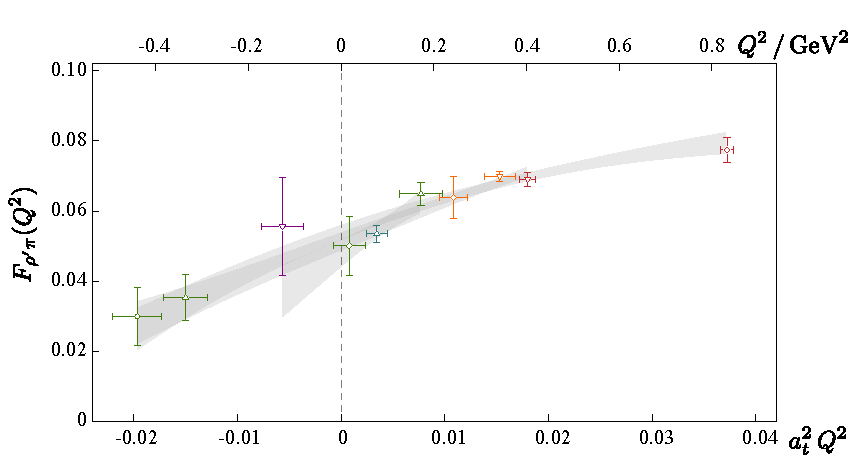
\includegraphics[width=0.8\linewidth]{figures/radTrans/rho_proj1_pion_proj0.pdf}
  \caption{First-excited $\rho$ transition to ground-state $\pi$ form-factor, $F_{\rho'\pi}(Q^2)$. Points have the same color and shape labeling presented in Figure~\ref{fig::rho_pi_transition}. Gray curves show fits used to interpolate to the photocoupling. \label{fig::rho1_pi_transition}}
  \end{centering}
\end{figure}
\clearpage
}




%%%%%%%%%%%%%%%%%%%%%%%%%%%%%%%%%%%%%%%%%%%%%%%%%%%%%%%%%%%%
\subsubsection{$\rho''\rightarrow \pi \gamma$ transition}

An extraction analogous to that presented in the previous subsection can be performed for the second-excited $\rho$ state, leading to the form-factor shown in Figure~\ref{fig::rho2_pi_transition}. Interpolating to $Q^2=0$ using a range of forms yields $F_{\rho'' \pi}(Q^2) = -0.016(3)$, which is smaller still than the $\rho' \to \pi \gamma$ photocoupling. The sign is somewhat arbitrary and would only have definite meaning were we to compare to other transitions involving the $\rho''$.

Within a simple $q\bar{q}$ bound-state model we might expect the $\rho''$ state to be dominated by a $^3\!D_1$ configuration (and indeed the operator overlaps presented in \cite{Dudek:2011bn} seem to suggest this), which would have a `hindered' structure in a transition to the ground-state $S$-wave pseudoscalar owing to the need for the current to provide a $D$-wave angular dependence, which appears only as a relativistic correction to the leading behavior. 

\afterpage{
\begin{figure}[htbp]
\begin{centering}
  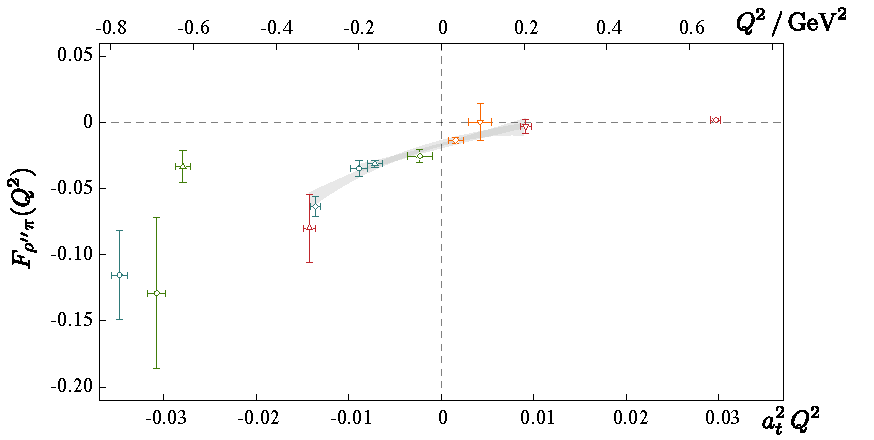
\includegraphics[width=0.8\linewidth]{figures/radTrans/rho_proj2_pion_proj0.pdf}
    \caption{ Second-excited $\rho$ transition to ground-state $\pi$ form-factor, $F_{\rho'' \pi}(Q^2)$. Points have the same color and shape labeling presented in Figure~\ref{fig::rho_pi_transition}. Gray curves show fits used to interpolate to the photocoupling. 
     \label{fig::rho2_pi_transition}}
       \end{centering}
\end{figure}
\clearpage
}




%%%%%%%%%%%%%%%%%%%%%%%%%%%%%%%%%%%%%%%%%%%%%%%%%%%%%%%%%%%%
\subsubsection{$\pi' \rightarrow \rho \gamma$ transition}

The first-excited pion may undergo a transition to the ground-state $\rho$. The results, extracted from $\Delta t = 20 \, a_t$ correlation functions, are presented in Figure~\ref{fig::pi1_rho0_transition}, along with a number of parameterizations used to interpolate a photocoupling of $F_{\pi' \rho}(0) = 0.18(2)$. Again we observe a significant suppression relative to the $\rho \to \pi \gamma$ case in line with this being a hindered transition.

\afterpage{
\begin{figure}[htbp]
\begin{centering}
  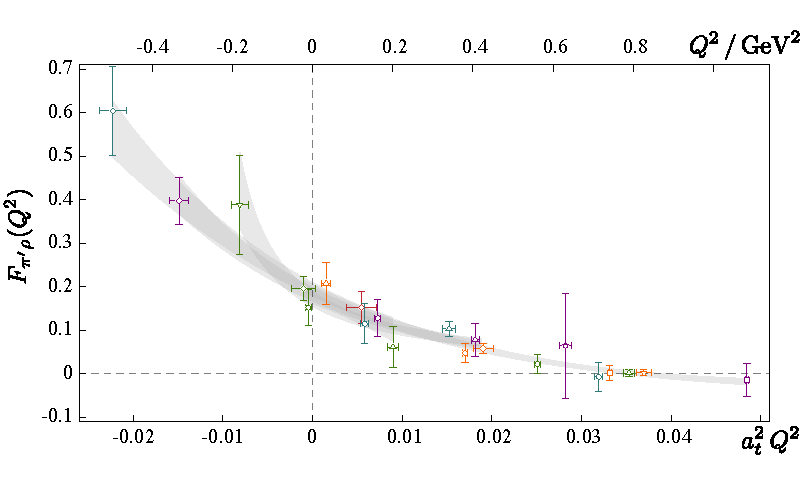
\includegraphics[width=0.8\linewidth]{figures/radTrans/rho_proj0_pion_proj1.pdf}
    \caption{First-excited $\pi$ transition to ground-state $\rho$, $F_{\pi' \rho}(Q^2)$. Gray curves show fits used to interpolate to the photocoupling. \label{fig::pi1_rho0_transition}}
  \end{centering}
\end{figure}
\clearpage
}







%%%%%%%%%%%%%%%%%%%%%%%%%%%%%%%%%%%%%%%%%%%%%%%%%%%%%%%%%%%%
\subsubsection{$\rho' \rightarrow \pi' \gamma$ transition}

This transition, which occurs between excited states, is not expected to be hindered in the case that the $\rho'$ and $\pi'$ are identified predominantly as the first radial excitations of the $\rho$ and $\pi$ respectively. As such we might expect a somewhat larger photocoupling than in previous subsections. We extracted the form-factor from optimized operator correlation functions with $\Delta t = 20 \,a_t$ obtaining the results presented in Figure~\ref{fig::rho1_pi1_transition}. Fits to the $Q^2$ dependence with a range of forms lead to an estimate of the photocoupling, $F_{\rho' \pi'}(Q^2) = 0.7(2)$, which, although not determined with high precision, is of comparable size to the $\rho \to \pi \gamma$ coupling. 

\afterpage{
\begin{figure}[htbp]
\begin{centering}
  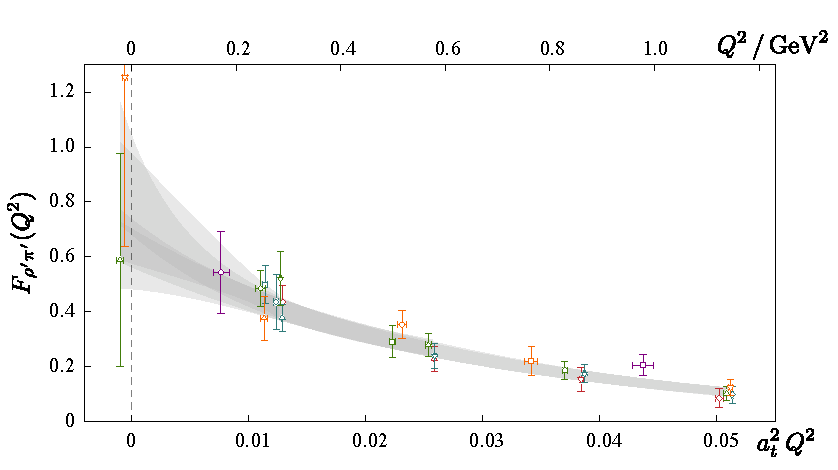
\includegraphics[width=0.8 \linewidth]{figures/radTrans/rho_proj1_pion_proj1.pdf}
      \caption{First-excited $\pi$ transition to first-excited $\rho$, $F_{\pi' \rho'}(Q^2)$. Gray curves show fits used to interpolate to the photocoupling. \label{fig::rho1_pi1_transition}}
        \end{centering}
\end{figure}
\clearpage
}




























